\section{Introduction}

\frame{
  \frametitle{Part of}
  \begin{figure}
    
\includegraphics[width=0.8\textwidth]{figures/madelogo}
  \end{figure}
  Workpackage 8: Hyperflexible Automation
  \pnote{Introducte. Joint venture to improve domestic manufactoring. Supply chain, QA and stuff.}
}
\frame{
  \frametitle{3D Vision}
  \begin{minipage}[t]{0.48\linewidth}
    \begin{itemize}
      \item Use readily available 3D sensors.
      \item Solve problems.
      \item Both industrial and academic.
    \end{itemize}
  \end{minipage}
  \begin{minipage}[t]{0.48\linewidth}
    \begin{figure}
      \includegraphics[width=1.0\linewidth]{figures/nrsfm_scanner}
    \end{figure}
  \end{minipage}
  \pnote{Wide availability of 3D sensors sparks this thesis. Solve problems industrial and academic. Specifically structured light.}
}

\begin{comment}
\frame{
  \frametitle{Commercial 3D Sensors}
  \begin{figure}
    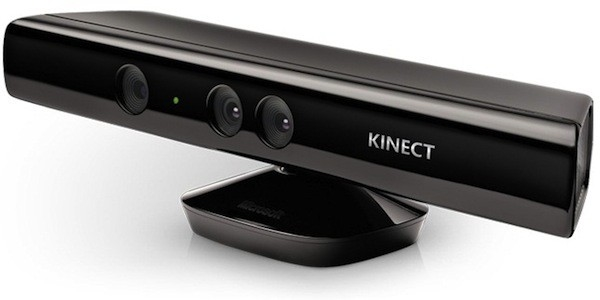
\includegraphics[width=0.35\linewidth]{figures/kinect}
    \hspace{2cm}
    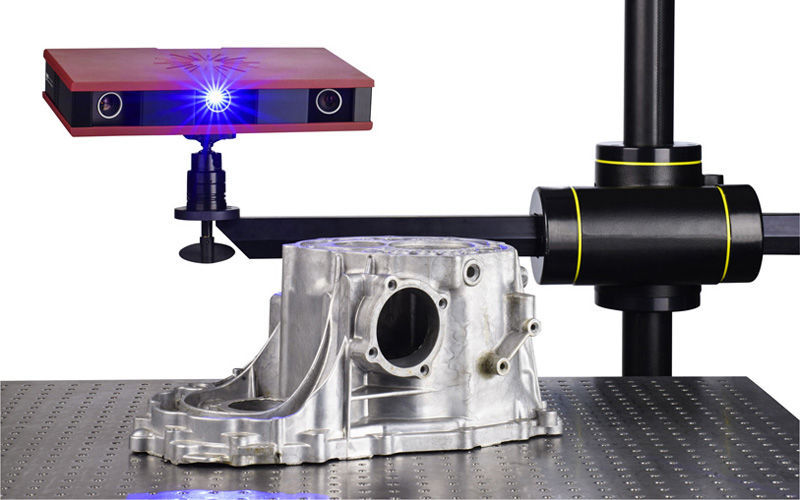
\includegraphics[width=0.35\linewidth]{figures/gom}
  \end{figure}
  \begin{figure}
    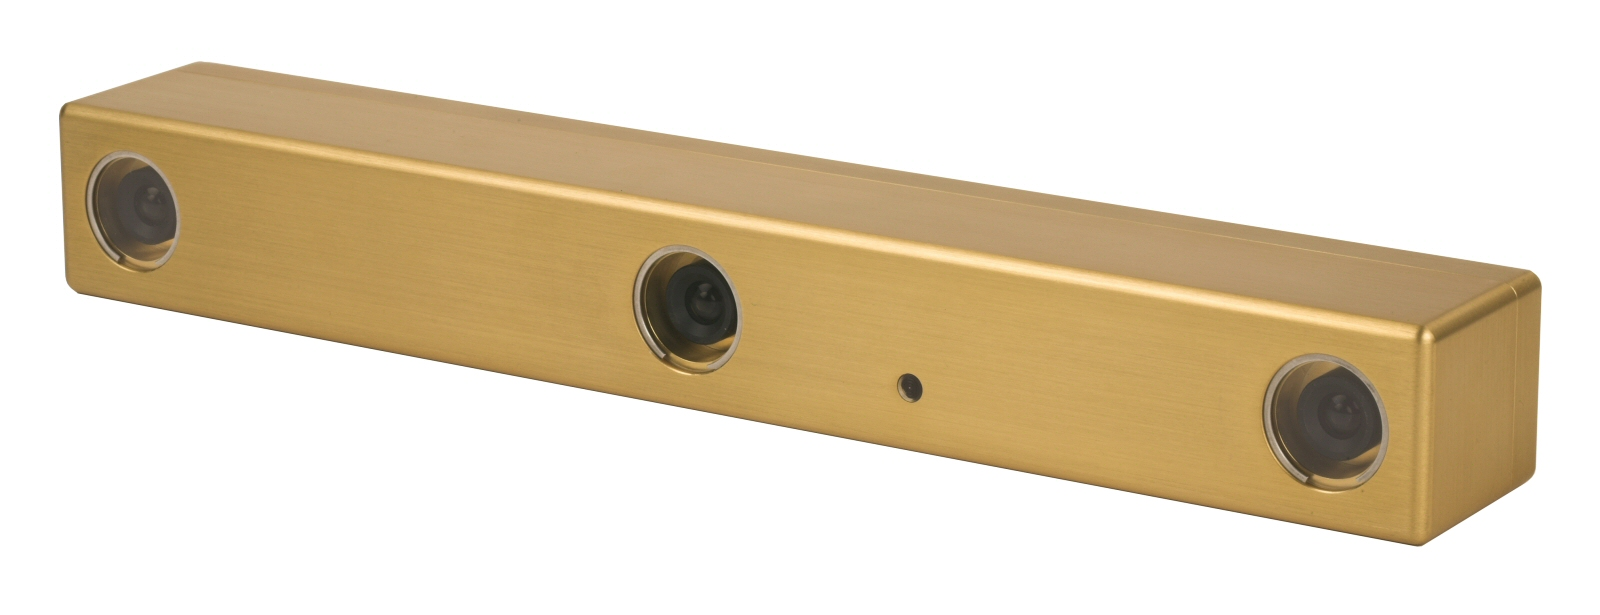
\includegraphics[width=0.35\linewidth]{figures/bumblebee}
    \hspace{2cm}
    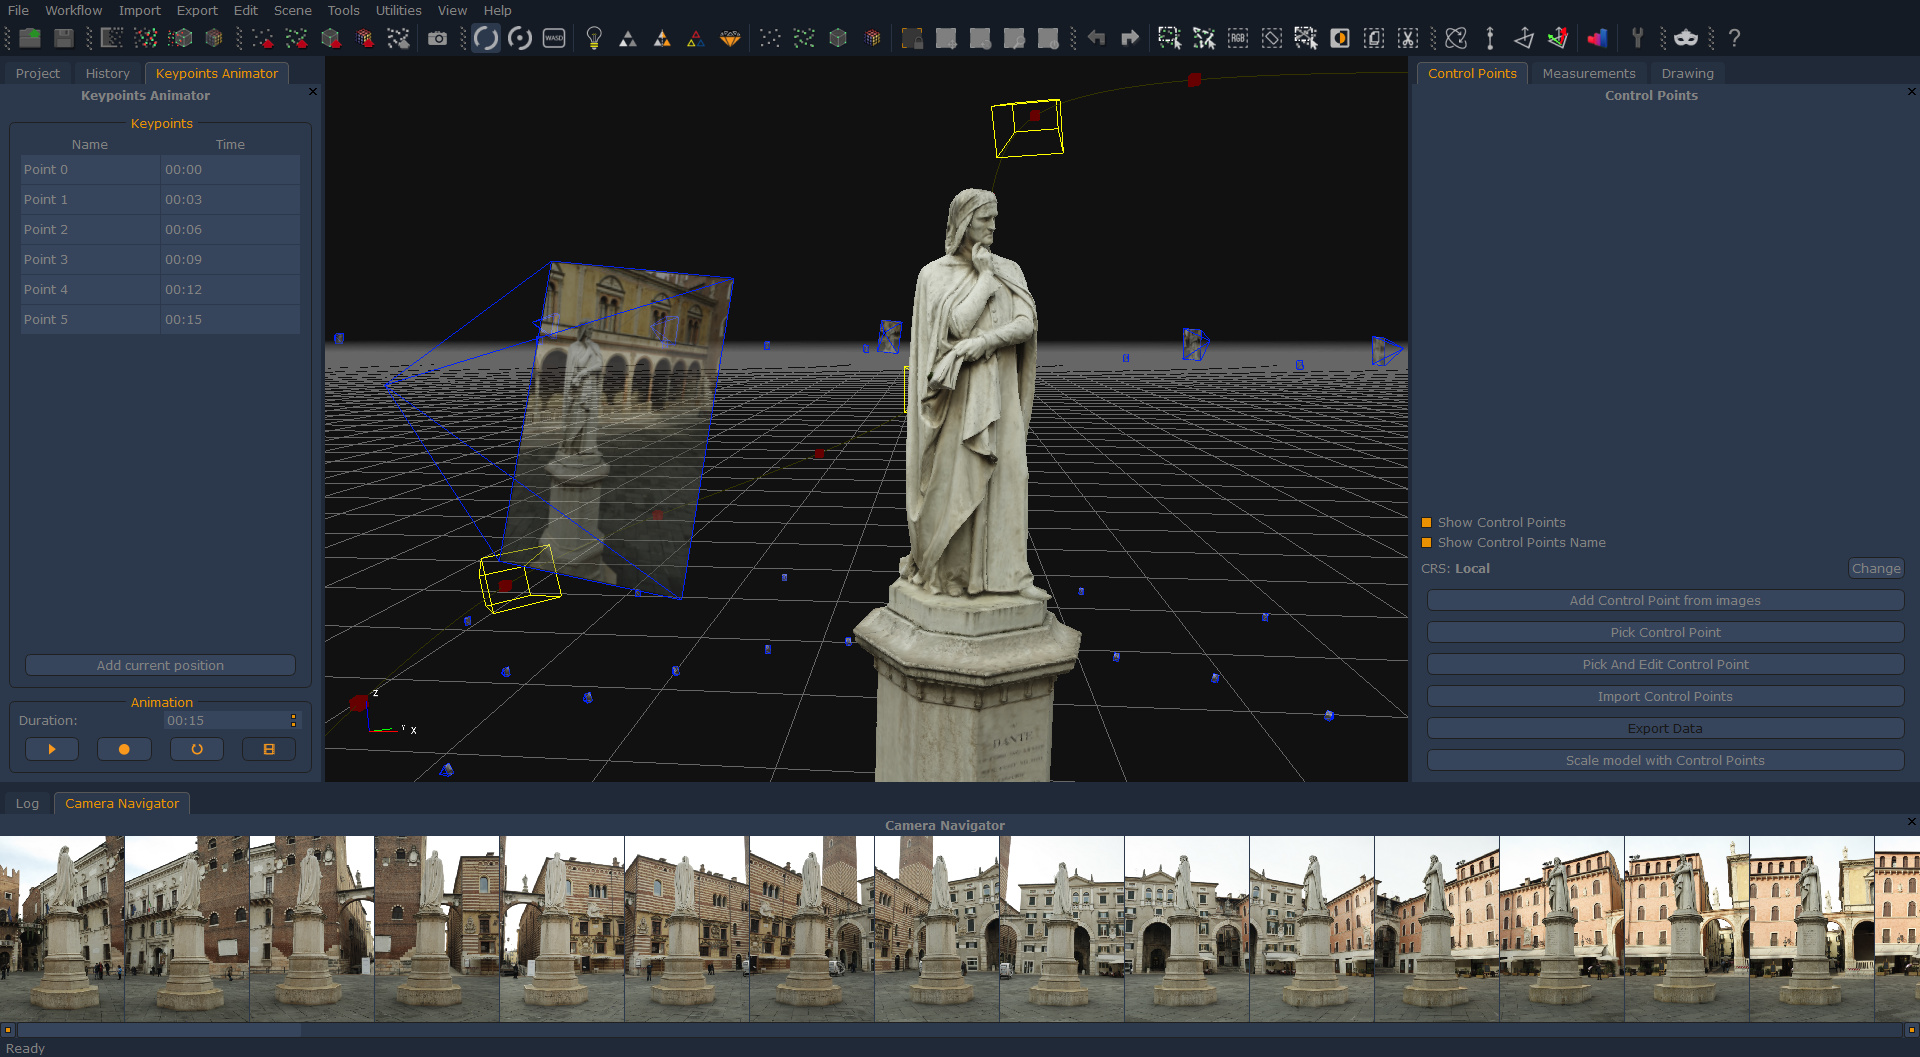
\includegraphics[width=0.35\linewidth]{figures/3df_zephyr_3_photogrammetry_statue}
  \end{figure}
}

\frame{
  \frametitle{3D Vision Application}
  \begin{figure}[t]
    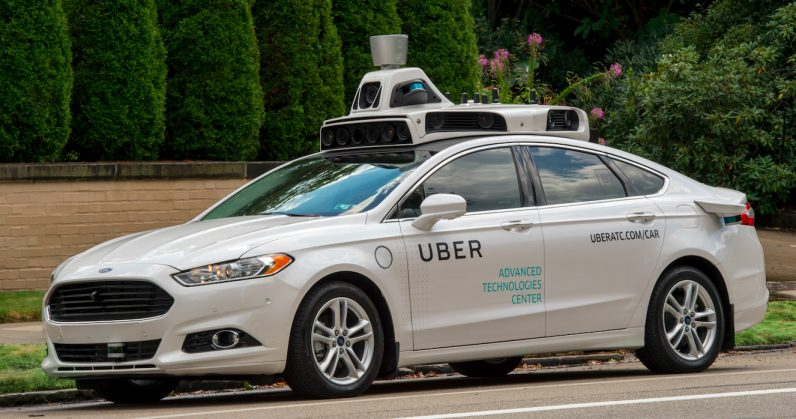
\includegraphics[width=0.47\linewidth]{figures/selfdriving}
    \hfill
    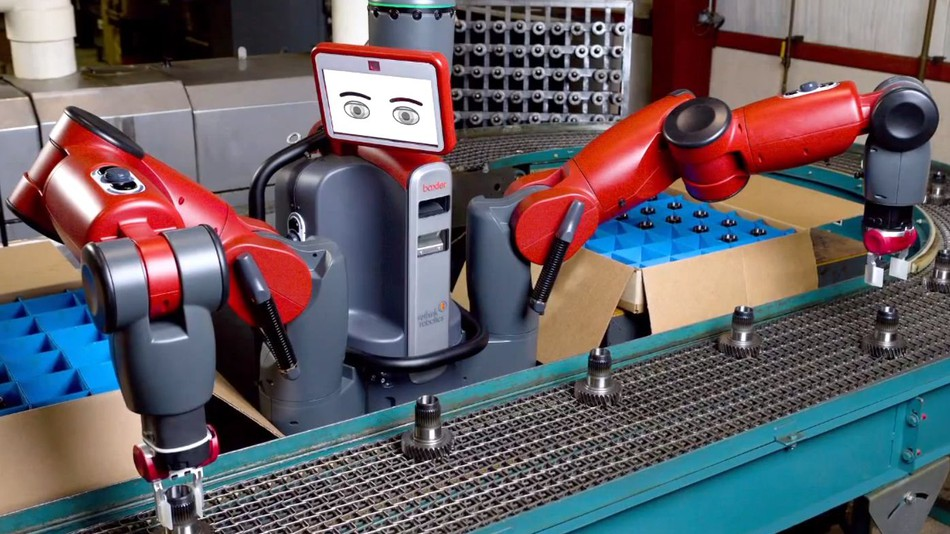
\includegraphics[width=0.47\linewidth]{figures/baxter}
  \end{figure}
}

\frame{
  \frametitle{Real-world application can be surprisingly tricky...}
  \begin{figure}
    \centering
    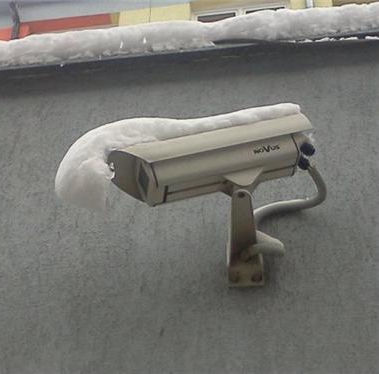
\includegraphics[height=0.65\textheight]{figures/icecam}
    \hfill
    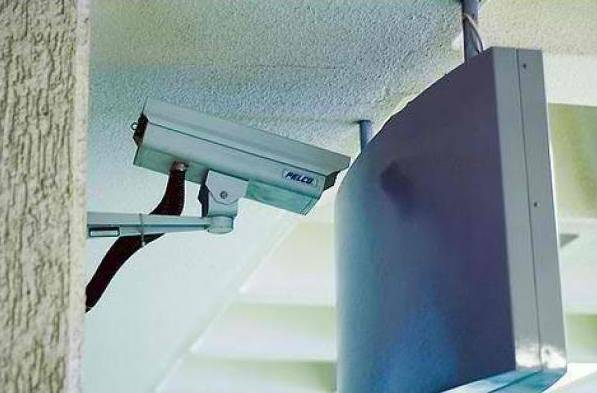
\includegraphics[height=0.65\textheight]{figures/failed2}
  \end{figure}
}
\end{comment}

\frame{
  \frametitle{Todays Topics}
  \tableofcontents
  \pnote{work exemplified by three studies.}
}
